
\section{Getting started}
\subsection{Zugangsberechtigung einholen / neues Passwort anfordern}

% Die Zugangsberechtigung zum CUBE PA erhalten Sie für das Projekt Zugkunft Waldenburgerbahn beim Gesamtleiter. Senden Sie
% eine E-Mail an folgende Adresse (Zeitpunkt der Aufschaltung wird noch bekanntgegeben):

Die Zugangsberechtigung zum CUBE PA erhalten Sie jeweils über den Projektverantwortlichen. Bei Fragen bezüglich den Zuständigkeiten oder dem Freischalten eines CUBE PA-Zugangs können Sie sich an folgende Email-Adresse wenden:

\vspace{\baselineskip}

% \href{mailto:cube.support@emchberger.ch}{\textstyleInternetlink{cube.support@emchberger.ch}}
{\color{red} cube.support@emchberger.ch}

\vspace{\baselineskip}

Falls Sie Ihr Passwort vergessen haben, können Sie auf der Login-Seite des CUBE PA mittels der Funktion 'Passwort vergessen' ein neues Passwort anfordern, resp. wird Ihnen ein Link zugestellt, mit welchem Sie ein neues Passwort setzen können. Bei Fragen können Sie sich ebenfalls an obige Email-Adresse wenden.

\vspace{\baselineskip}

Aus Sicherheitsgründen empfehlen wir per Email erhaltene Passwörter sofort zu ändern.

\subsection{Internetverbindung}

Eine funktionierende Internetverbindung ist eine Voraussetzung für die Benutzung des CUBE PA. Offline Arbeiten wird nicht unterstützt, da alle Daten auf einem Server gespeichert sind.

\vspace{\baselineskip}

Falls Sie beim Benutzen des CUBE PA unerwartete Probleme feststellen, beachten Sie das Statussymbol der Verbindung unten rechts auf dem Bildschirm. Falls dieses rot ist, ist die Internet-Verbindung unterbrochen. Falls Ihnen dies während dem Erfassen von Daten passiert, versuchen Sie, die Internetverbindung wieder herzustellen und wenn dies gelingt, klicken Sie auf 'Übernehmen', um die im lokalen Arbeitsspeicher des CUBE PAs vorhandenen Daten zu sichern. Falls es auf die Schnelle nicht gelingt die Internet-Verbindung wieder herzustellen, verlassen Sie den CUBE ProjectAssistant nicht, und schalten Sie den Computer nicht aus. Suchen Sie einen anderen Standort, wo Sie eine Internet-Verbindung herstellen
können und sobald eine solche vorhanden ist, klicken Sie auf 'Übernehmen'.

\vspace{\baselineskip}

\textbf{Status der Verbindung:}

\vspace{\baselineskip}

\begin{tabular}{c | p{14cm} l} %{cl}

\vspace{+1pt}	

\includegraphics[height=12pt] {/Icons/online.jpg} & Sie haben eine Internet-Verbindung und sind im CUBE PA angemeldet. \\
\vspace{+1pt}	

\includegraphics[height=12pt]{/Icons/offline.jpg} & Die Internet-Verbindung ist unterbrochen oder der CUBE PA-Server ist vorübergehend nicht erreichbar. \\
\vspace{+1pt}	

\includegraphics[height=12pt]{/Icons/abgemeldet.jpg} & Sehen Sie kein Statussymbol haben Sie eine Internet-Verbindung, sind aber nicht im CUBE PA angemeldet. \\

% 
\includegraphics[height=12pt]{/Icons/BlaueWolke_Blitz.jpg} & Sie haben eine Internet-Verbindung, sind aber nicht in CUBE PA angemeldet \\

\end{tabular}

\vspace{\baselineskip}

Falls Sie den CUBE PA verlassen während die Internet-Verbindung unterbrochen ist, gehen die zuletzt erfassten Daten verloren.

\subsection{CUBE PA starten}

% Benutzerspezifisch

Der Zugriff auf CUBE PA erfolgt über die folgende Adresse:

\vspace{\baselineskip}

{\color{red} http://www.cubetools.ch/}

\vspace{\baselineskip}

Sie gelangen auf die Startseite der CUBE Tools:

\begin{figure}[H]
\center{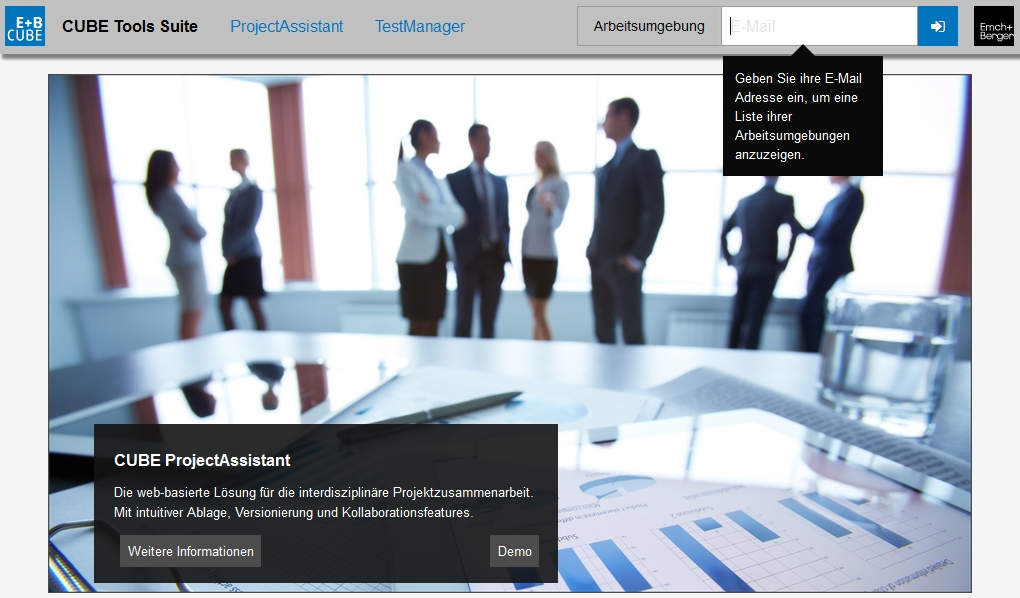
\includegraphics[width=.9\linewidth]{../chapters/02_GettingStarted/pictures/2-3_Einstiegsseite.jpg}}
\caption{Die Einstiegsseite für den CUBE PA}
% \label{fig:speciation}
\end{figure}

Geben Sie oben rechts im Fenster Ihre Email-Adresse ein und klicken Sie auf den blauen Pfeil-Button neben der eingegebenen Email-Adresse:

\begin{figure}[H]
\center{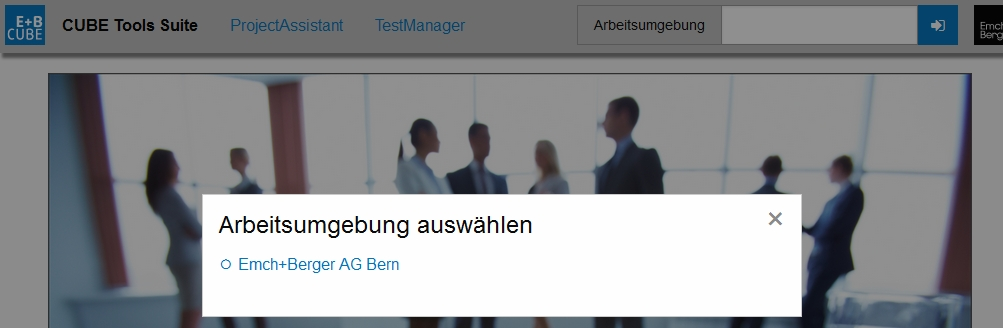
\includegraphics[width=.8\linewidth]{../chapters/02_GettingStarted/pictures/2-3_Arbeitsumgebung_auswaehlen.jpg}}
\caption{Die Arbeitsumgebung auswählen}
% \label{fig:speciation}
\end{figure}

Es werden sämtliche Arbeitsumgebungen angezeigt, bei welchen Sie registriert sind. Im Suchfeld können Sie nach der gewünschten Arbeitsumgebung suchen. Klicken Sie auf die entsprechende Arbeitsumgebung. Sie gelangen nun auf die Anmeldemaske:

\begin{figure}[H]
\center{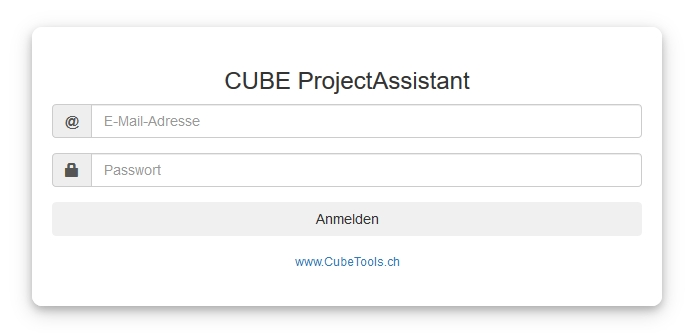
\includegraphics[width=0.5\linewidth]{../chapters/02_GettingStarted/pictures/2-3_CUBEPA_Anmeldung.jpg}}
\caption{An CUBE PA anmelden}
% \label{fig:speciation}
\end{figure}

Geben Sie Ihre Email-Adresse und das Passwort ein. Nach Klick auf 'Anmelden' erscheint die persönliche Übersicht.

\vspace{\baselineskip}

\textbf{Hinweis:} Wenn Sie noch nicht registriert sind, können Sie mit Klick auf den Link 'Registrierung' einen Zugang beantragen. Füllen Sie das Formular aus und klicken Sie auf den Button 'Registrieren'.

\vspace{\baselineskip}

\textbf{Hinweis:} Haben Sie in Ihrem Browser gültige Zugangsdaten (Email-Adresse und Passwort) hinterlegt, werden Sie direkt in CUBE PA eingeloggt.

\subsection{Passwort ändern}
\label{bkm:Ref434828103}

Aus Sicherheitsgründen empfehlen wir Ihnen jedes Passwort, dass Sie per Email erhalten haben, sofort zu ändern. Klicken Sie dazu oben links im Bildschirm auf ihren Namen. Es wird ein Menü geöffnet, welches Ihnen ermöglicht sich beim CUBE PA abzumelden, das Passwort zu ändern oder das vorliegende Handbuch zu öffnen oder zu speichern.

\begin{figure}[H]
\center{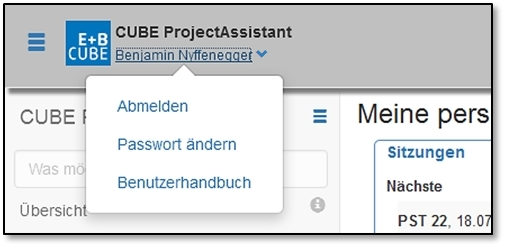
\includegraphics[width=0.5\linewidth]{../chapters/02_GettingStarted/pictures/2-4_Passwort_aendern.jpg}}
\caption{Das Passwort ändern}
% \label{fig:speciation}
\end{figure}

Mit Klick auf 'Passwort ändern' erscheint eine Maske, in der Sie einmal das alte Passwort und zweimal das neue Passwort eingeben müssen:

\begin{figure}[H]
\center{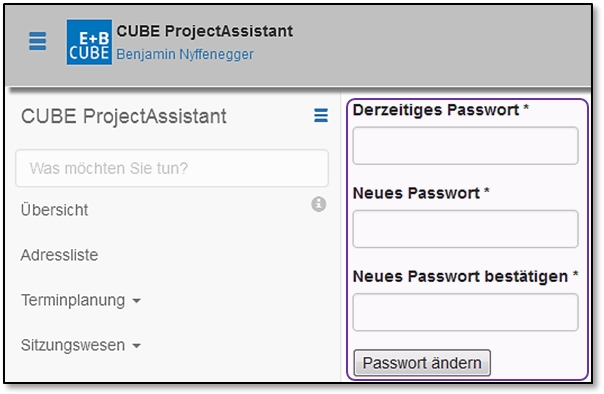
\includegraphics[width=0.5\linewidth]{../chapters/02_GettingStarted/pictures/2-4_Passwort_Eingabe.jpg}}
\caption{Neues Passwort eintragen}
% \label{fig:speciation}
\end{figure}

Sobald Sie die Schaltfläche 'Passwort ändern' anklicken, gilt das neue Passwort.

\subsection{Die wichtigsten Menüs, Schaltflächen, Symbole und Hinweise in Kürze}

Die Bedienung des CUBE PA orientiert sich an der gebräuchlichen Bedienung von Internet-Applikationen. Wer regelmässig ein Smartphone oder ein Tablet benutzt, wird sich im CUBE PA schnell zurechtfinden.

\vspace{\baselineskip}

In diesem Kapitel werden die wichtigsten Menüs, Schaltflächen und Symbole erläutert, die in allen Teilen des CUBE PA erscheinen und immer die gleiche Bedeutung haben.

\pagebreak

\subsubsection{Menüs}

\begin{figure}[H]
\center{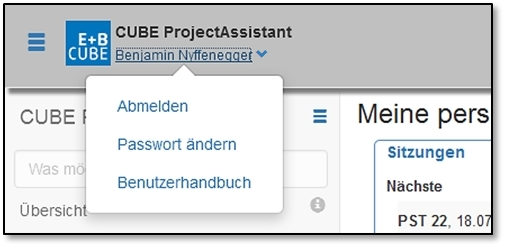
\includegraphics[width=0.5\linewidth]{../chapters/02_GettingStarted/pictures/2-4_Passwort_aendern.jpg}}
\caption{Das Eingangsmenü}
% \label{fig:speciation}
\end{figure}


Oben links sehen Sie jeweils, wer im CUBE PA angemeldet ist. Mit Klick auf den Namen öffnen sich weitere Optionen. Das Wechseln des Passwortes wurde oben beschrieben (Kapitel \ref{bkm:Ref434828103}). Sie haben mit Klick auf 'Benutzerhandbuch' die Möglichkeit das vorliegende Handbuch per pdf zu öffnen oder zu speichern. Wenn Sie auf 'Abmelden' klicken, verlassen Sie den CUBE PA ohne Umschweife, ausser Sie hätten neu erfasste Daten noch nicht gespeichert. In diesem Fall erscheint eine Warnung:

\begin{figure}[H]
\center{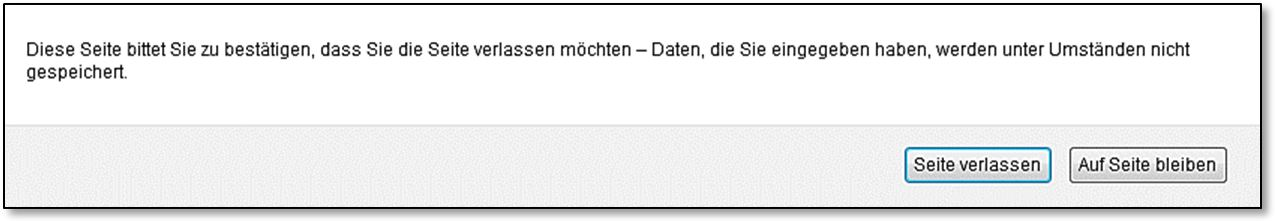
\includegraphics[width=1\linewidth]{../chapters/02_GettingStarted/pictures/2-5-1_Browsermeldung.jpg}}
\caption{Browser-Warnung}
% \label{fig:speciation}
\end{figure}
\begin{small}
Der Inhalt dieser Meldung ist abhängig vom verwendeten Browser (hier Firefox) und somit nicht beeinflussbar.
\end{small}

\vspace{\baselineskip}

Sie können das Verlassen des CUBE PA abbrechen (Auf Seite bleiben) und die noch nicht gespeicherten Daten sichern, indem Sie auf 'Übernehmen' klicken.

\vspace{\baselineskip}

\pagebreak

Links befindet sich das Hauptmenü:

\vspace{\baselineskip}

\begin{wrapfigure}[20]{l}{6.5cm}   % [x] Wie manche Zeile soll sich um die Grafik "brechen"
  \vspace{-35pt}      % Grundwert war 20; mit 30 schön oben beim Text ausgerichtet
  \begin{center}
    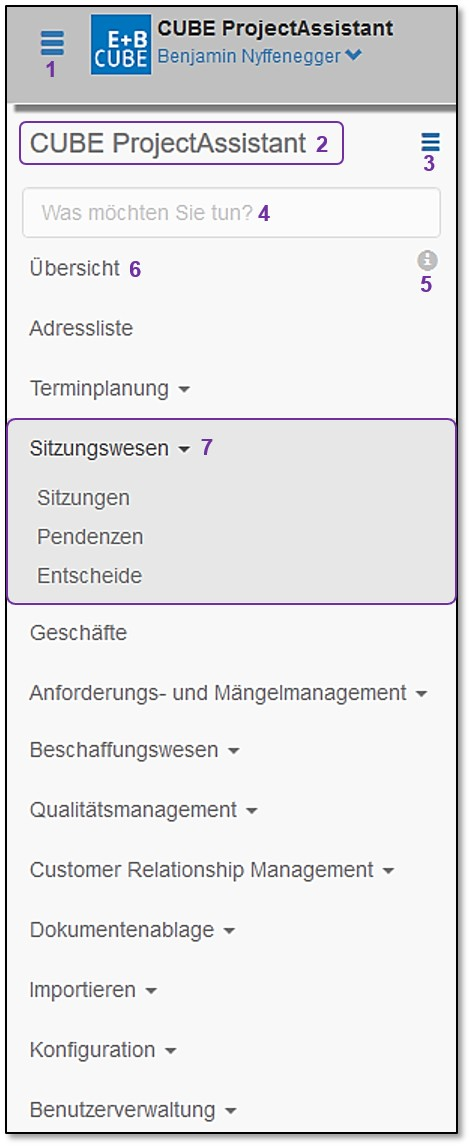
\includegraphics[width=1\linewidth]{../chapters/02_GettingStarted/pictures/2-5-1_Menu_Uebersicht.jpg}
  \end{center}
  \vspace{-20pt}
  \caption{Das Menü verwenden}
  \vspace{-10pt}
\end{wrapfigure}

Das Menü ermöglicht die Auswahl sämtlicher Modulen, für welche Sie berechtigt sind. Entsprechend kann sich die Abbildung zu Ihrem Menü unterscheiden. Ebenso ist es möglich, dass sich innerhalb eines Menü die Unterpunkte (z. B. ein zusätzlicher Punkt 'Externe Sitzungen' beim Sitzungswesen) unterscheiden, da kundenspezifisch weitere Menüpunkte konfiguriert werden können. Die Grundfunktionen sind aber dieselben. Mit Klick auf das Menü-Icon \col{(1)} können Sie jeweils das gesamte Menü ein- und ausblenden. Damit gewinnen Sie bei Bedarf eine grössere Arbeitsfläche in Ihrem Browser. \\
Die Bezeichnung unter \col{(2)} zeigt Ihnen die aktuelle Arbeitsumgebung an. Mit Klick auf das Icon \col{(3)} können Sie die Arbeitsumgebung direkt wechseln. 

\vspace{\baselineskip}

\begin{raggedleft}
\hspace{80mm} 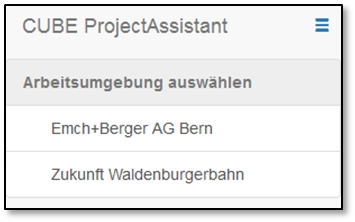
\includegraphics[height=40mm]{../chapters/02_GettingStarted/pictures/2-5-1_Arbeitsumgebung_wechseln.jpg}
\end{raggedleft}

\vspace{\baselineskip}

Es werden Ihnen natürlich nur diejenigen Arbeitsumgebungen angezeigt, für welche Sie eine Berechtigung haben. Mit Klick auf die gewünschte Arbeitsumgebung kommen Sie zum Anmeldefenster der entsprechenden Arbeitsumgebung. Falls Sie an diesem Tag (ohne den Computer neu gestartet zu haben) eine Arbeitsumgebung bereits mal geöffnet hatten, gelangen Sie ohne Anmeldung wieder in die gewünschte Umgebung. Mit Klick auf das gleiche Symbol \col{(3)} schliessen Sie diese Auswahl wieder. 

\vspace{\baselineskip}

Ein zentrales Werkzeug ist das Such-Feld 'Was möchten Sie tun?' \col{(4)}. Hilfreich für eine zielführende und effektive Anwendung sind die Informationen, welche Sie mit dem Info-Icon \col{(5)} erhalten:

\begin{figure}[H]
\center{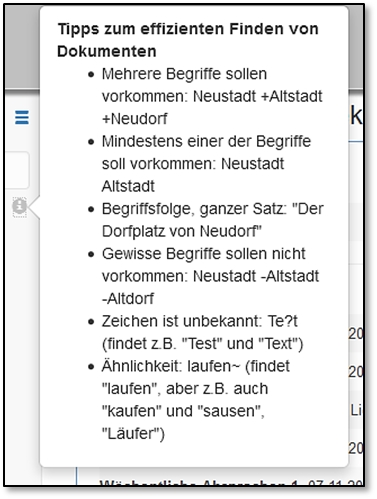
\includegraphics[width=0.35\linewidth]{../chapters/02_GettingStarted/pictures/2-5-1_Hilfe_zu_Suche.jpg}}
\caption{Tipps für eine effektive Suche}
% \label{fig:speciation}
\end{figure}

Wenn Sie irgendwo in das Browserfenster klicken, schliesst das Info-Fenster wieder. Geben Sie ins Such-Feld \col{(4)} den oder die gewünschten Begriff/e ein. CUBE PA durchsucht alle Menüthemen und Einträge, sowie auch Inhalte von hochgeladenen Dokumenten (z.B. Word und PDF). \\

\textbf{Wichtig zu beachten} ist, dass PDF-Dokumente nur durchsucht werden können, wenn es sich auch um integrierten Text und nicht um Bilder handelt. Wurde ein Text gescannt und als Bild in einem PDF gespeichert, wird dieser Inhalt nicht durchsucht.\\

\begin{wrapfigure}[14]{r}{7cm}   % [x] Wie manche Zeile soll sich um die Grafik "brechen"
  \vspace{-30pt}      % Grundwert war 20; mit 30 schön oben beim Text ausgerichtet
  \begin{center}
    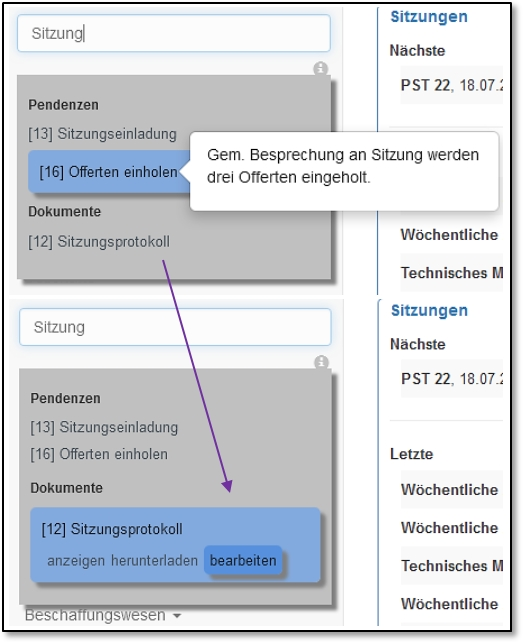
\includegraphics[width=0.8\linewidth]{../chapters/02_GettingStarted/pictures/2-5-1_Such_Ergebnisse.jpg}
  \end{center}
  \vspace{-20pt}
  \caption{Suchergebnisse verwenden}
  \vspace{-10pt}
\end{wrapfigure}

Alle gefundenen Übereinstimmungen werden nun angezeigt:

\begin{compactitem}
	\item Unter dem Stichwort wurden Einträge bei den Pendenzen und bei den Dokumenten gefunden.
	\item Fahren Sie mit der Maus über einen Eintrag der Pendenzen, erscheinen Details zu 'Offerten einholen'.
	\item Unter anderen Themen, hier unter Dokumente, haben Sie die Möglichkeit das gefundene Dokument (hier ein Sitzungsdokument) anzeigen zu lassen, herunterzuladen oder zu bearbeiten. Dazu fahren Sie mit der Maus über die gewünschte Option. Diese wird dann hervorgehoben und mit einem Mausklick ausgeführt.
\end{compactitem}

\vspace{\baselineskip}

Mit dem Menüpunkt 'Übersicht' \col{(6)} gelangen Sie immer wieder zurück auf die persönliche Übersichtsseite. Sind unter einem Menüpunkt weitere Unterpunkte vorhanden, wird dies mit einem kleinen Dreieck angezeigt. Wenn Sie auf den Titel klicken, werden die Untermenüs sichtbar \col{(7)}. Der Hauptpunkt 'Sitzungswesen' ist selbst nicht verlinkt. Mit erneutem Klick darauf schliessen die Unterpunkte wieder.

\vspace{\baselineskip}

Das Haupt-Menü gibt Zugang zu den verschiedenen Modulen des CUBE PA. Je nach erteilten Benutzerrechten sind nicht alle Rubriken für alle Benutzer sichtbar und zugänglich.

\begin{itemize}
\item
\textbf{Übersicht}: zeigt die für Sie relevanten Sitzungen, Pendenzen, Dokumente und Beschaffungen an.
\item
\textbf{Adressliste: }Anzeigen der erfassten Adressen mit Filterfunktion. Hier können auch neue Einträge (Personen und Organisationen) angelegt werden.
\item
\textbf{Terminplanung}: Anzeigen und Filtern von Terminplänen.
\item
\textbf{Sitzungswesen}: Anzeigen und Bearbeiten von Sitzungseinladungen, Sitzungsprotokollen, Pendenzen und
Entscheiden.
\item
\textbf{Geschäfte}: Unterstützung für ein einfach zu erfassendes, strukturiertes Projektjournal.
\item
\textbf{Anforderungs- und Mängelmanagement}: Unterstützung bei der Abnahme von Projekten. Überblick über offene Mängel und Nachbesserungen.
\item
\textbf{Beschaffungswesen}: Abwickeln von Beschaffungen, von der Ausschreibung bis zum Vertragsabschluss.
\item
\textbf{Qualitätsmanagement}: Zugriff auf Dokumente über Risikomanagement und Nahtstellen. Hier können Sie auch ein Projekthandbuch oder andere Handbücher erstellen.
\item
\textbf{Customer Relationship Management}: Das CRM (Customer Relationship Management) ermöglicht Ihnen effizient Veranstaltungen (Anlässe, Präsentationen und Schulungen) zu koordinieren.
\item
\textbf{Dokumentenablage}: Dokumenten-Management mit Online-Ansicht. Geänderte Dokumente werden mit einer neuen Versionsnummer abgelegt.
\item
\textbf{Importieren}: Importieren von Daten (Adresslisten, Termine und Geschäfte).
\item
\textbf{Konfiguration}: Hier werden die Inhalte der Auswahllisten festgelegt und angepasst.
\item
\textbf{Benutzerverwaltung}: Verwalten von Benutzern, Teams und Gruppen.
\end{itemize}

% bishierher

\subsubsection{Schaltflächen}

Die folgenden Schaltflächen kommen immer wieder vor:

\vspace{\baselineskip}

% 2.8, 12

\begin{tabular}{|c | p{10cm}|l} %{cl}
\hline
\raisebox{-1\totalheight}{
\includegraphics[height=20pt]{/Icons/B_Erstellen.jpg}} & Erstellen: Durch Klicken auf diese Schaltfläche speichern Sie einen neu erfassten Datensatz zum ersten Mal, was Ihnen dann die Möglichkeit zur weiteren Bearbeitung öffnet. \\
\hline
\raisebox{-1\totalheight}{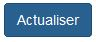
\includegraphics[height=20pt]{/Icons/B_Uebernehmen.jpg}} & Übernehmen: Wenn Sie auf diese Schaltfläche klicken, bewirken Sie, dass kürzlich erfasste oder geänderte Daten, die bis jetzt nur im Arbeitsspeicher ihres Computers vorhanden sind, auf dem Server gesichert werden. \\
\hline
\raisebox{-1\totalheight}{
\includegraphics[height=20pt]{/Icons/Lupe_s.jpg}} & Lupe: Durch Klicken auf diese Lupe filtern Sie eine Liste, nachdem Sie in den Feldern auf der ersten Zeile der Liste die Filterkriterien ausgewählt oder einen Suchbegriff eingegeben haben. \\
\hline
\raisebox{-1\totalheight}{
\includegraphics[height=20pt]{/Icons/FilterLoeschen.jpg}} & Filter löschen: Durch Klicken auf dieses Symbol werden sämtliche Eingaben in den Suchfeldern gelöscht. \\
\hline
\raisebox{-1\totalheight}{
\includegraphics[height=16pt]{/Icons/weitereSeiten.jpg}} & Blättern in Liste: mit dieser Schaltfläche können Sie in einer Liste vorwärts oder zurückblättern, in dem Sie auf 'Weiter' oder 'Zurück' klicken, oder eine bestimmte Seite auswählen, indem Sie auf die Seitennummer klicken. Falls die Liste mehr als fünf Seiten umfasst, werden nicht alle Seitennummern angezeigt. Klicken Sie auf 'Weiter' oder 'Zurück' bis die gewünschte Seite angewählt werden kann.  \\
\hline
\end{tabular}

\begin{figure}[H]
\center{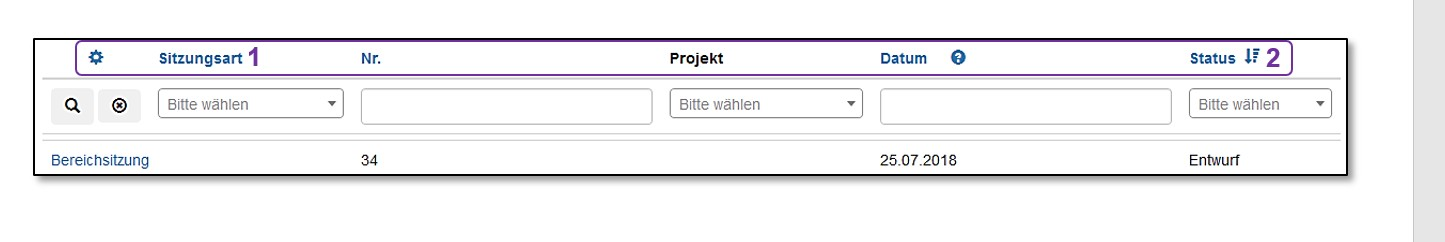
\includegraphics[width=1\linewidth]{../chapters/02_GettingStarted/pictures/2-5-2_Listen_sortieren.jpg}}
\caption{Spalten: Inhalt sortieren}
% \label{fig:speciation}
\end{figure}


Zusätzlich haben alle in blau erscheinenden Spaltentitel von Listen die Wirkung einer Schaltfläche \col{(1)}. Durch Klicken auf einen Spaltentitel sortieren Sie die
Liste in aufsteigender Reihenfolge bezüglich dieser Spalte. Durch erneutes Klicken auf den Spaltentitel kehren Sie die Reihenfolge um. Das kleine Dreieck 
\includegraphics[height=10pt]{/Icons/sortieren.jpg} \col{(2)} zeigt einerseits nach welcher Spalte sortiert wird (hier nach 'Status') und andererseits wie die Reihenfolge der Sortierung ist: (Sortierung A {\textgreater} Z 
\includegraphics[height=10pt]{/Icons/Status_down.jpg} resp. Z {\textgreater} A 
\includegraphics[height=10pt]{/Icons/Status_up.jpg}).

\pagebreak
\subsubsection{Symbole}
\label{bkm:Ref443039356}
Die folgenden Symbole haben überall im CUBE PA dieselbe Bedeutung. Solche Schaltflächen und Textlinks wechseln in der Regel die Farbe, wird der Mauszeiger darüber bewegt. (Gilt nicht für die Statussymbole der Verbindung). 

\begin{tabular}{|c|p{14cm}|} %{cl}
\hline
\raisebox{-0.5\totalheight}{
\includegraphics[height=12pt]{/Icons/online.jpg}} & Unten links im Fenster sehen Sie die grünen Pfeilen. Dies bedeutet, Sie haben eine Internet-Verbindung und sind in CUBE PA angemeldet. \\

\includegraphics[height=12pt]{/Icons/offline.jpg} & Werden die Pfeile rot angezeigt, ist die Internetverbindung unterbrochen oder der CUBE PA-Server vorübergehend nicht erreichbar. \\

\includegraphics[height=12pt]{/Icons/abgemeldet.jpg} & Sehen Sie keine Pfeile, sind Sie aktuell an keiner Arbeitsumgebung in CUBE PA angemeldet. \\
\hline
\raisebox{-1\totalheight}{
\includegraphics[height=12pt]{/Icons/Plussymbol.jpg}} & Dieses Pluszeichen steht jeweils oben links im Fenster. Durch Klicken können Sie einen neuen Datensatz erstellen (z.B. eine neue Sitzungseinladung erfassen). \\
\hline
\raisebox{-1\totalheight}{
\includegraphics[height=12pt]{/Icons/Filter.jpg}} & Mit Klick auf dieses Symbol öffnen sich weitere Filtermöglichkeiten. Diese Filtereinstellungen lassen sich abspeichern und später wieder aufrufen. \\
\hline
\raisebox{-1\totalheight}{
\includegraphics[height=12pt]{/Icons/Nadelsymbol.jpg}} & Mit Klick auf das Nadelsymbol wird die Google-Maps ein- respektive wieder ausgeblendet. \\
\hline
\raisebox{-1\totalheight}{
\includegraphics[height=12pt]{/Icons/Listensymbol_zurueck.jpg}} & Mit diesem Listensymbol kehren Sie zurück zur Übersicht. Meist wird dieses Symbol angezeigt, wenn Sie sich mittels Lupe (Ansicht) oder Stift (Bearbeiten) in einem einzelnen Datensatz befinden. \\
\hline
\raisebox{-1\totalheight}{
\includegraphics[height=12pt]{/Icons/SpaltenEinst.jpg}} & Mit Klick auf dieses Konfigurationssymbol können Sie für Ihre Ansicht Spalten ein- und ausblenden. Für nicht benötigte Spalten nehmen Sie das Häkchen raus. \\
\hline
\raisebox{-1\totalheight}{
\includegraphics[height=12pt]{/Icons/Stift.jpg}} & Der Bleistift steht jeweils in der linke Ecke neben einem Feld \col{(1)} in einer Liste. Sie können nach einem Klick auf den Bleistift den Inhalt dieses Feldes bearbeiten.   
\includegraphics[height=14pt]{../chapters/02_GettingStarted/pictures/2-5-3_Datum_edit.jpg}\\
\hline
\raisebox{-1\totalheight}{
\includegraphics[height=12pt]{/Icons/Gutzeichen.jpg}} & Wurden in einer Eingabemaske Änderungen vorgenommen, werden diese mit Klick auf das Gutzeichen gespeichert. \\
\hline
\raisebox{-1\totalheight}{
\includegraphics[height=12pt]{/Icons/Bearbeiten.jpg}} & Bleistift in Quadrat (klein): Mit einem Klick auf dieses Symbol öffnen Sie eine Maske, die das Bearbeiten sämtlicher Felder des entsprechenden Eintrages erlaubt. \\
\hline
\raisebox{-1\totalheight}{
\includegraphics[height=12pt]{/Icons/Pluszeichen.jpg}} & Pluszeichen: Durch einen Klick auf ein Pluszeichen können Sie einen neuen Eintrag in einer Liste erstellen, z.B. einen zusätzlichen Teilnehmer für eine Sitzungseinladung erfassen, Anhänge hinzufügen oder einer Person / Gruppe zusätzlich Berechtigungen erteilen. \\
\hline
\raisebox{-1\totalheight}{
\includegraphics[height=12pt]{/Icons/Lupe.jpg}} & Lupe: Dieses Symbol steht unmittelbar bei einer Zeile / einem Eintrag in einer Liste. Mit einem Klick darauf öffnen Sie eine Maske, die das Lesen des Inhalts aller Felder des entsprechenden Datensatzes erlaubt. \\
\hline
\raisebox{-1\totalheight}{
\includegraphics[height=12pt]{/Icons/Blattsymbol.jpg}} & Blatt mit Eselsohr oben rechts: Dieses Symbol kommt in einem Listenfeld vor. Durch einen Klick auf das Symbol können Sie eine PDF-Datei generieren. Der Spaltentitel sagt aus, welchen Inhalt das PDF-Dokument aufweist. \\
\hline
\end{tabular}

\pagebreak

\begin{tabular}{|c|p{14cm}|} %{cl}
\hline
\raisebox{-1\totalheight}{
\includegraphics[height=12pt]{/Icons/VertPfeile.jpg}} & Gegenläufige vertikale Pfeile: Wenn Sie dieses Symbol mit gedrückt gehaltener linker Maustaste packen, können Sie diese Zeile innerhalb einer Liste nach oben oder unten verschieben und so die Reihenfolge der Einträge verändern. \\
\hline
\raisebox{-1\totalheight}{
\includegraphics[height=12pt]{/Icons/Muelltonne.jpg}} & Mülltonne: Durch einen Klick auf dieses Symbol können Sie eine Zeile einer Liste samt den zugehörigen Daten löschen. Z.B. löschen Sie so die Angaben zu einer Beilage und die Beilage selbst. Es erscheint eine Sicherheitsmeldung „Entfernen?“ Mit der Bestätigung auf „OK“ veranlassen Sie das Löschen der Daten. \\
\hline
\raisebox{-1\totalheight}{
\includegraphics[height=12pt]{/Icons/Kreuzchen.jpg}} & Kreuzchen in Feldern: Durch Klicken auf das Kreuzchen am rechten Rand eines Felds löschen Sie den Inhalt eines Feldes mit Auswahlliste. \\
\hline
\raisebox{-1\totalheight}{
\includegraphics[height=12pt]{/Icons/Pfeil_rechts.jpg}} & Horizontales Pfeilsymbol: Mit einem Klick darauf klappen Sie einen Inhalt aus (machen ihn sichtbar). \\
\hline
\raisebox{-1\totalheight}{
\includegraphics[height=12pt]{/Icons/Pfeil_unten.jpg}} & Vertikales Pfeilsymbol: Mit einem Klick darauf klappen Sie einen Inhalt ein (machen ihn unsichtbar). \\
\hline
\raisebox{-1\totalheight}{
\includegraphics[height=12pt]{/Icons/Verknuepfen.jpg}} & Ein bestehendes Dokument aus der Dokumentenablage verknüpfen. \\
\hline
\raisebox{-1\totalheight}{
\includegraphics[height=12pt]{/Icons/ListeGenerieren.jpg}} & Mittels dieses Icons können Sie aus verschiedenen Ansichten / Modulen eine Excelliste generieren. \\
\hline
\end{tabular}

\subsubsection{Warnungen und Hinweise}

\textbf{Webseite verlassen ohne Daten zu speichern:} \\
Wenn Sie im CUBE PA Daten-Felder ausgefüllt haben und ohne Klick auf 'Übernehmen' oder 'Erstellen' die aktuelle Seite verlassen wollen, erscheint folgende Meldung: 

\begin{figure}[H]
\center{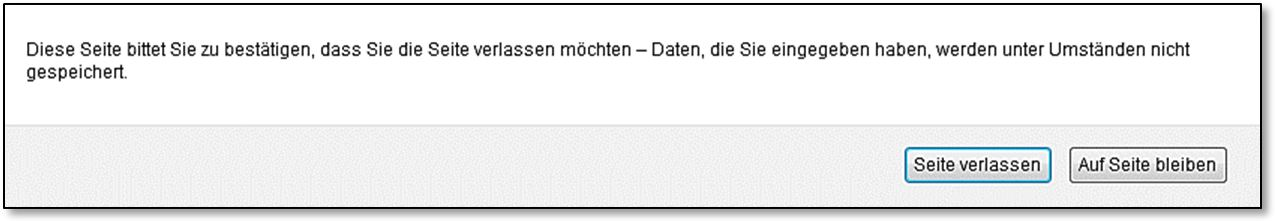
\includegraphics[width=1\linewidth]{../chapters/02_GettingStarted/pictures/2-5-1_Browsermeldung.jpg}}
\caption{Browser-Warnung}
% \label{fig:speciation}
\end{figure}
\begin{small}
Der Inhalt dieser Meldung ist abhängig vom verwendeten Browser (hier Firefox) und somit nicht beeinflussbar.
\end{small}

\vspace{\baselineskip}

Sie haben die Möglichkeit durch Klick 'Auf Seite bleiben' zurückzukehren und durch Klick auf 'Übernehmen' oder 'Erstellen' die Daten zu sichern. Andererseits gehen die Daten verloren.

\vspace{\baselineskip}

\textbf{Pflichtfelder:}\\
Bei der Eingabe von Daten gibt es Pflichtfelder (mit einem * markiert), welche zwingend ausgefüllt werden müssen. Wird ein solches Pflichtfeld übersehen, erscheint folgende Meldung:

\begin{figure}[H]
\center{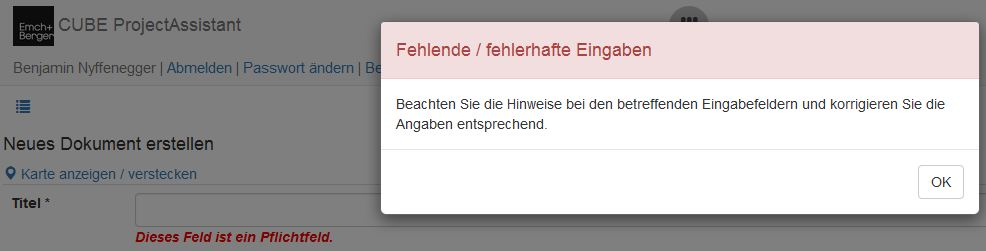
\includegraphics[width=1\linewidth]{../chapters/02_GettingStarted/pictures/2-5-4_WarnungPflichfelder}}
\caption{Warnung Eingabe bei Pflichtfeld}
% \label{fig:speciation}
\end{figure}

Mit roter Schrift wird dann jeweils das Feld bezeichnet, welches ausgefüllt werden muss (Dieses Feld ist ein Pflichtfeld). Die Hinweismeldung kann mittels 'OK' weggeklickt werden. Erst nach einer Eingabe ist es möglich die Daten zu speichern und z.B. ein neues Dokument anzulegen. 

\vspace{\baselineskip}

\textbf{Speichern/Übernehmen während dem Hochladen von Dateien:}\\
Laden Sie in der Dokumentenablage eine grössere Datei hoch, kann das einige Zeit in Anspruch nehmen. Wollen Sie während dem Hochladen bereits die Eingaben speichern, erscheint eine Meldung, dass noch gerade Dateien hochgeladen werden. Warten Sie bis das Hochladen abgeschlossen ist (Fortschritt = 100 \%), danach können Sie auch 'Übernehmen' klicken. Meldung:

\begin{figure}[H]
\center{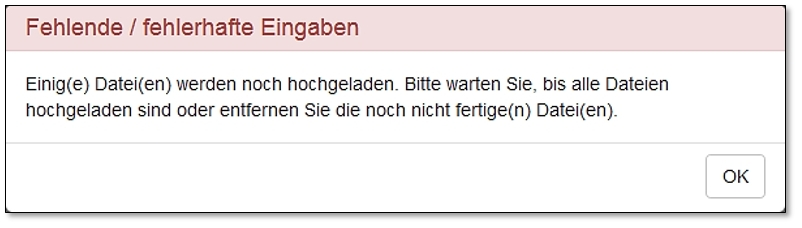
\includegraphics[width=.6\linewidth]{../chapters/02_GettingStarted/pictures/2-5-4_MeldungHochladen.jpg}}
\caption{Warnung beim Speichern während dem Hochladen einer Datei}
% \label{fig:speciation}
\end{figure}

\pagebreak
\subsection{Übersicht der Filteranwendung / Suche in den verschiedenen Modulen}

In den verschiedenen Übersichten (z.B. Adressliste, Dokumentenablage, Sitzungswesen etc.) finden Sie immer wieder die gleichen Bedienungsschritte der Filter- und Suchfunktionen. In gewissen Modulen kann es in der Funktionalität leichte Abweichungen geben. 

\vspace{\baselineskip}

Im Folgenden die wichtigsten Funktionen und Bedienelemente der Übersicht:

\begin{figure}[H]
\hspace*{-2.3cm}
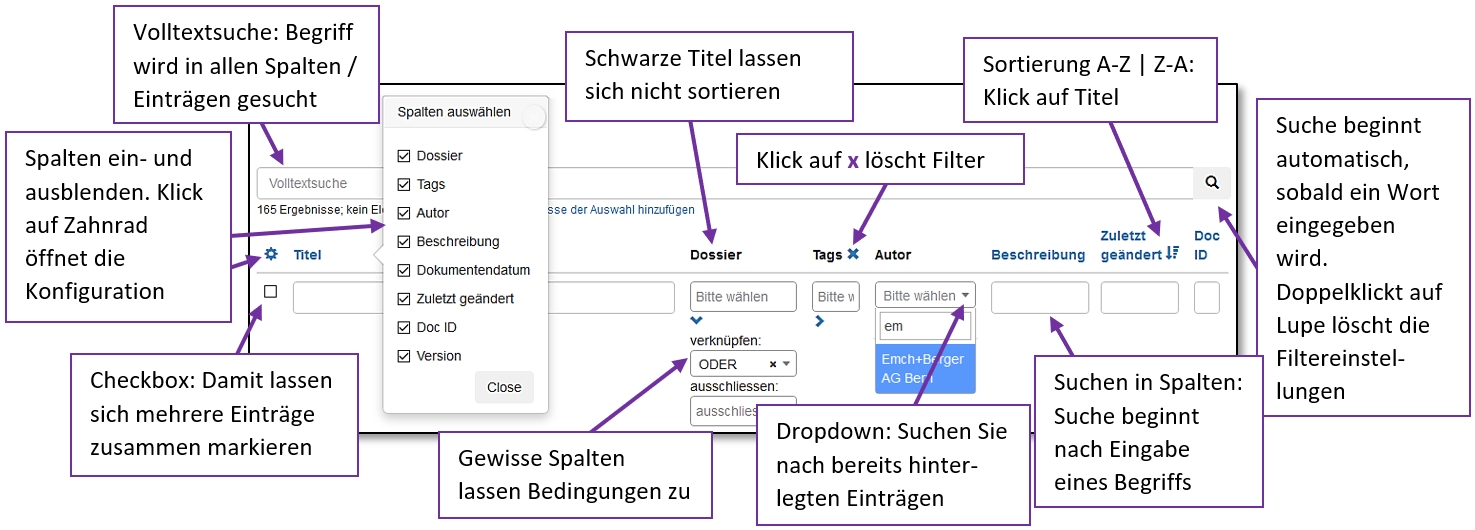
\includegraphics[width=1.25\linewidth]{../chapters/02_GettingStarted/pictures/uebersicht_Bedienung}
\caption{Bedienelemente in der Übersicht}
% \label{fig:speciation}
\end{figure}


% \begin{figure}[H]
% \center{\includegraphics[width=1.2\linewidth]{../chapters/02_GettingStarted/pictures/uebersicht_Bedienung}}
% \caption{Bedienelemente in der Übersicht}
% \label{fig:speciation}
% \end{figure}

\textbf{Wichtigste Funktionen:}

\vspace{\baselineskip}

\begin{compactitem}
	\item \textbf{Automatische Suche:} Sobald Sie ein Suchwort in die Volltextsuche oder ein Spaltensuchfeld eingeben, beginnt CUBE die Ansicht zu filtern. Mit Doppelklick auf die Lupe wird der Filter zurückgesetzt und sämtliche Suchbegriffe werden gelöscht.
	\item \textbf{Spalten ein- und ausblenden:} Mit Klick auf \includegraphics[height=12pt]{/Icons/SpaltenEinst.jpg} öffnet die Spaltenkonfiguration, bei welcher Sie zur besseren Übersicht Spalten ein- und ausblenden können.
	\item \textbf{Sortieren:} Mit Klick auf einen blauen Spaltentitel wird diese Spalte von A-Z oder Z-A sortiert. Die sortierte Spalte ist am entsprechenden Sortierungsicon erkennbar \includegraphics[height=12pt]{/Icons/sort_up.jpg} oder \includegraphics[height=12pt]{/Icons/sort_down.jpg}.
		\item \textbf{Mehrfachauswahl:} Mit Klick auf das Kästchen links von einem Eintrag (\includegraphics[height=12pt]{/Icons/checkbox_leer.jpg}) lassen sich mehrere Einträge zusammen auswählen und anschliessend versenden, drucken (via Reprozentrum) oder favorisieren.
	\item \textbf{Weitere Funktionen:} Bei einigen Spalten ist es möglich, mittels Bedingungen 'und' / 'oder' Suchbegriffe zu verknüpfen oder auszuschliessen. Die Spalten können verschiedene Feldeigenschaften aufweisen: Freitext, Dropdown mit in der Datenbank hinterlegten Einträgen, Datumsfelder etc.
	\item \textbf{Suchoptionen:} Bei Dropdown-Spalten können Sie mehrere Begriffe auswählen, entweder in dem Sie nacheinander nach bestimmten begriffen suchen oder mit gedrückter CTRL-Taste mehrere Begriffe auswählen. Zudem können Sie auswählen, ob Sie alle Einträge anzeigen lassen wollen, bei welchen die ausgesuchte Spalte 'leer' oder gerade 'nicht leer' sind. Wählen Sie dazu im Dropdown-Menü \{leer\} resp. \{nicht leer\} aus. 
\end{compactitem}	

\vspace{\baselineskip}

Für weitere Eigenheiten in der Bedienung der entsprechenden Modulen beachten Sie die Beschreibungen in den entsprechenden Kapitel dieses Handbuches.

% \pagebreak
\subsection{Benachrichtigung bei Veränderungen der Dateneinträgen und Dokumenten}
\label{bkm:Ref2018080601}

CUEB PA bietet in einigen Modulen (Dokumentenablage, Pendenzen, Anforderungen, Beschaffungswesen etc.) die Möglichkeit, Benachrichtigungsregeln zu erstellen und so die Veränderungen von Einträgen und Dokumenten zu verfolgen. Wird ein 'beobachtetes' Dokument oder ein entsprechender Eintrag verändert, erhalten Sie eine Email. Dadurch sind Sie immer auf dem Laufenden und wissen, wann von Ihnen wieder eine Aktion erfolgen kann oder Daten aktualisiert wurden.

\begin{figure}[H]
\center{\includegraphics[width=1\linewidth]{../chapters/02_GettingStarted/pictures/getS_Benachrichtigung.jpg}}
\caption{Benachrichtigung erstellen}
% \label{fig:speciation}
\end{figure}

Eine Benachrichtigungsregel kann überall dort erstellt werden, wo das Auge-Symbol ersichtlich ist. Mit Klick auf das Auge-Symbol \includegraphics[height=12pt]{/Icons/Auge_g.jpg} \col{(1)} gelangen Sie zur Konfigurationsseite:

\begin{figure}[H]
\center{\includegraphics[width=1\linewidth]{../chapters/02_GettingStarted/pictures/getS_BenachRegelErstellen.jpg}}
\caption{Benachrichtigungsregel erstellen}
% \label{fig:speciation}
\end{figure}

Klicken Sie auf das Plussymbol \includegraphics[height=12pt]{/Icons/Pluszeichen.jpg}, nun können Sie eine neue Regel erstellen.

Die Konfiguration im Überblick:

\begin{compactitem}
	\item \includegraphics[height=12pt]{/Icons/Pluszeichen.jpg} \col{(1)}: Sie können mehrere Regeln erstellen, wiederholen Sie den Konfigurationsschritt.
	\item \includegraphics[height=12pt]{/Icons/checkbox_markiert.jpg} \col{(2)}: Standardmässig wird ein einzelner Datensatz beobachtet. Wenn Sie das Gutzeichen in der Box entfernen, gilt die Regel für alle Datensätze (z.B. für alle Pendenzen).
	\item \includegraphics[height=12pt]{/Icons/Muelltonne.jpg} \col{(3)}: Eine erstellte Regel können Sie auch wieder löschen.
	\item \includegraphics[height=12pt]{/Icons/Gutzeichen.jpg} \col{(4)}: Einstellungen werden mit dem Gutzeichen gespeichert.
	\item \includegraphics[height=12pt]{/Icons/Refresh.jpg} \col{(5)}: Mit dem Refresh-Symbol aktualisieren Sie die Einträge.
	\item \includegraphics[height=12pt]{/Icons/X_Button.jpg} \col{(6)}: Oben rechts schliessen Sie das Fenster ohne die Einträge / Regeln zu speichern.
	\item \col{(a)}: Wählen Sie das gewünschte Benachrichtigungsintervall aus.\\
	\textbf{Hinweis:} Falls mehrere Änderungen innerhalb einer Minuten gemacht werden, erhalten Sie nicht für jede Änderung eine Email. Die kleinste Zeiteinheit ist eine Minute.
	\item \col{(b)}: In der Spalte 'Beobachtete Felder' können Sie die gewünschten Felder auswählen, für welche die Benachrichtigungsregel gültig sein soll. Wie unter \col{(c)} beschrieben, werden sämtliche Felder eines oder aller Datensätze beobachtet, wenn das Feld nicht ausgefüllt wird.
\end{compactitem}

\begin{figure}[H]
\center{\includegraphics[width=1\linewidth]{../chapters/02_GettingStarted/pictures/getS_BenachOptionen.jpg}}
\caption{Benachrichtigungsregel erstellen}
% \label{fig:speciation}
\end{figure}

\textbf{Farblegende:}\\
\includegraphics[height=12pt]{/Icons/Auge_g.jpg}: Wurde keine Benachrichtigungsregel auf einen Datensatz angewandt, ist das Auge grau.\\
\includegraphics[height=12pt]{/Icons/Auge_r.jpg}: Wurde eine Benachrichtigungsregel für diesen Datensatz erstellt, ist das Auge rot.\\
\includegraphics[height=12pt]{/Icons/Auge_b.jpg}: Wurde bei einem Datensatz ausgewählt, dass sämtliche Datensätze beobachtet werden sollen, ist das Auge blau.\\

\vspace{\baselineskip}

\textbf{Hinweis}: Die Möglichkeit sämtliche Datensätze zu beobachten, ist mit Bedacht anzuwenden.

\pagebreak
\subsection{Statussystem} % Workflow
\label{bkm:Ref2018073101}

Verschiedene Module von CUBE PA verwenden ein Statussystem. Beispielsweise folgt das Beschaffungswesen einem Workflow (verschiedene Status), welcher zusammen mit dem Kunden definiert wurde.

Andere Module enthalten ebenfalls ein Statussystem, mit welchem ein Workflow definiert werden kann. Im Folgenden wird die Anwendung eines generischen Statussystems beschrieben. In Folgenden Modulen ist aktuell ein Statussystem implementiert:

\vspace{\baselineskip}

\begin{compactitem}
	\item \textbf{Anforderungs- und Mängelmanagement:} Anforderungen, Mängel und Arbeitspakete
	\item \textbf{Dokumentenablage:} Dossier und Dokumente
\end{compactitem}

\vspace{\baselineskip}

\textbf{Statussystem in der Dokumentenablage:}

\vspace{\baselineskip}

Im Betrachtungs- oder Bearbeitungsmodus eines Dokuments finden Sie oben das Statussymbol \includegraphics[height=12pt]{/Icons/status_aendern.jpg} \col{(1)}: 

\begin{figure}[H]
\center{\includegraphics[width=.75\linewidth]{../chapters/02_GettingStarted/pictures/getS_StatusAufrufen.jpg}}
\caption{Einen Status aufrufen}
% \label{fig:speciation}
\end{figure}

Im folgenden Fenster kann der Status geändert werden:

\begin{figure}[H]
\center{\includegraphics[width=.85\linewidth]{../chapters/02_GettingStarted/pictures/getS_StatusAendern.jpg}}
\caption{Ein Status ändern}
% \label{fig:speciation}
\end{figure}

Oben links sehen Sie für welches Dokument Sie den Status ändern \col{(1)}. Die Status sind vorgegeben und können per Dropdown ausgewählt werden \col{(2)} (Das Statussystem kann grundsätzlich an betriebliche Workflows angepasst werden). Geben Sie einen Grund für den Statuswechsel an \col{(3)}. Sie haben bei einem Statuswechsel auch die Möglichkeit Dokumente zu verlinken. Klicken Sie dazu auf das Linksymbol \includegraphics[height=12pt]{/Icons/link.jpg} \col{(4)} (Das gewünschte Dokument muss vorgängig in der Dokumentenablage erfasst werden.). Wurden sämtliche Angaben gemacht, können Sie den Statuswechsel mit 'Übernehmen' \col{(5)} abschliessen. Mit Klick auf \includegraphics[height=12pt]{/Icons/X_Button.jpg} \col{(6)} oben rechts können Sie das Fenster ohne Daten zu speichern, verlassen.

\vspace{\baselineskip}

\textbf{Dateien verlinken:}

\begin{figure}[H]
\center{\includegraphics[width=1\linewidth]{../chapters/02_GettingStarted/pictures/getS_LinkHinzufuegen.jpg}}
\caption{Ein Dokument beim Statuswechsel verlinken}
% \label{fig:speciation}
\end{figure}

Tippen Sie Suchbegriffe ins Feld 'Datei*'. Im Anschluss wählen Sie gewünschte Version des Dokumets aus oder wählen die Option '\includegraphics[height=12pt]{/Icons/checkbox_leer.jpg} Immer die neuste Version referenzieren'. Ergänzen Sie nach Bedarf die Informationen für das verlinkte Dokument und klicken Sie auf 'Übernehmen' \col{(5)}, um den Vorgang abzuschliessen.

\vspace{\baselineskip}

\textbf{Statushistorie:}\\
Im Betrachtungsmodus \includegraphics[height=12pt]{/Icons/Lupe.jpg} eines Eintrages sehen Sie unten an der Seite die Statushistorie:

\begin{figure}[H]
\center{\includegraphics[width=1\linewidth]{../chapters/02_GettingStarted/pictures/getS_StatusHistorie.jpg}}
\caption{Die Statushistorie}
% \label{fig:speciation}
\end{figure}

Mit Klick auf das \includegraphics[height=12pt]{/Icons/Pfeil_rechts_g.jpg}-Symbol wird die Statushistorie \col{(1)} angezeigt, mit erneutem Klick auf den Pfeil nach unten \includegraphics[height=12pt]{/Icons/Pfeil_rechts_g.jpg}-Symbol wird die Statushistorie angezeigt, mit erneutem Klick auf den Pfeil nach unten \includegraphics[height=12pt]{/Icons/Dropdown.jpg} wird die Statushistorie wieder zugeklappt.\\
In der Statushistorie sehen Sie wann durch wen einen Status geändert wurde. Ebenso ist der Kommentar ersichtlich. Wurde bei einem Statuswechsel eine Datei verknüpft, wird diese hier auch aufgelistet \col{(2)} und mit einem Klick auf den Link lässt sich die Datei öffnen oder speichern.

\subsection{Benutzerdefinierte Übersichten und Felder}

\textbf{Übersichten / Dashboards}

\vspace{\baselineskip}

\begin{figure}[H]
\center{\includegraphics[width=.75\linewidth]{../chapters/02_GettingStarted/pictures/getSUebersicht.jpg}}
\caption{Die persönliche Projektübersicht}
% \label{fig:speciation}
\end{figure}

Die 'Persönliche Projektübersicht' kann an individuelle Bedürfnisse angepasst werden. Es können sogenannte Kacheln (Sitzungswesen, Pendenzen, Pläne etc.) hinzugefügt oder zur besseren Übersicht weggelassen werden.

\vspace{\baselineskip}

Nebst der 'Persönlichen Projektübersicht' können weitere Übersichten hinzugefügt werden. Es lassen sich in Form eines Dashboards Diagramme oder Tabellen darstellen:

\begin{figure}[H]
\center{\includegraphics[width=.75\linewidth]{../chapters/02_GettingStarted/pictures/getSDashboard.jpg}}
\caption{Konfigurierbares Dashboard}
% \label{fig:speciation}
\end{figure}

Die Diagramme geben beispielsweise eine Übersicht über den aktuellen Verarbeitungsstand von Rechnungen wieder. Wie viele Rechnungen besitzen welchen Zustand (Status). Tabellarisch lassen sich diese Rechnungen auflisten, mit einem Klick gelangen Sie in den Betrachtungsmodus einer Rechnung. Mit einem weiteren Klick können Sie den Status der Rechnung verändern (\includegraphics[height=12pt]{/Icons/Status_aendern.jpg}) oder die Rechnung mit einem Klick auf \includegraphics[height=12pt]{/Icons/bearbeiten.jpg} bearbeiten.

\vspace{\baselineskip}

Nebst obigen Darstellungsarten lassen sich häufig benutzte und gespeicherte Filter (aus der Dokumentenablage, aus dem Anforderungsmanagement etc.) als Schnellzugriffe anzeigen. 

\vspace{\baselineskip}

\pagebreak
\textbf{Formularfelder}

\vspace{\baselineskip}

In den verschiedenen Modulen von CUBE PA (Anforderungsmanagement, Dokumentenablage etc.) können nebst den Standard-Formularfeldern benutzerdefinierte Felder hinzugefügt werden. CUBE PA lässt sich mit beliebig vielen Feldern ergänzen:

\vspace{\baselineskip}

\begin{compactitem}
	\item \textbf{Freitextfelder:} Es können eine grössere Anzahl Zeichen / Text eingegeben und formatiert werden.
	\item \textbf{Mehrfachauswahl:} Diese Felder greifen auf hinterlegte Daten zu und lassen den Benutzer eine Mehrfachauswahl treffen.
	\item \textbf{Einzelauswahl:} Dieses Feld ist dem Mehrfachauswahlfeld ähnlich, jedoch kann nur ein Datensatz ausgewählt werden. 
	\item \textbf{Checkboxen:} Checkboxen sind Auswahlboxen, welche simpel aktiviert oder deaktiviert werden können (mit einem Gutzeichen).
	\item \textbf{Datum:} Durch dieses Feld wird ein Datum ausgewählt.
\end{compactitem}

\vspace{\baselineskip}

\textbf{Hinweis:} Die Konfiguration einer Übersicht / Dashboards oder das Hinzufügen von benutzerdefinierten Feldern erfordert die Supportleistung des CUBE Teams. Bei weiteren Fragen wenden Sie sich an den CUBE-Support: {\color{red} cube.support@emchberger.ch}

\pagebreak
\subsection{CUBE PA auf mobilen Endgeräten (Smartphones, Tablets)}

CUBE PA kann auch auf mobilen Endgeräten wie Smartphones und Tablets verwendet werden. CUBE PA erkennt, dass es sich um ein mobiles Gerät handelt und schaltet automatisch auf die 'mobile' Ansicht um. Diese beinhaltet eine etwas abweichende Darstellung sowie angepasste Menüführung (siehe unten). Wird jedoch mit Tablets gearbeitet, auf welchen ein reguläres Windows-Betriebssystem installiert ist (z.B. Win 8.1 / Win 10 auf Microsoft Surface), wird die Ansicht nicht umgestellt, entsprechend lässt sich CUBE PA aktuell nicht oder nur umständlich mit Touch-Eingaben bedienen.


\begin{figure}[H]
\center{\includegraphics[width=1\linewidth]{../chapters/02_GettingStarted/pictures/2-6_Mobile_Ansicht.jpg}}
\caption{CUBE PA - mobile Ansicht}
% \label{fig:speciation}
\end{figure}

\vspace{\baselineskip}

\begin{tabular}{p{7cm} l} %{cl}
CUBE PA auf einem iPad: \newline Angepasstes Menü und Auswahl- \newline fenster für Touch-Eingaben. & \raisebox{-.6\totalheight}{\includegraphics[width=.5\linewidth]{../chapters/02_GettingStarted/pictures/2-6_iPad_Sitzungen.jpg}}\\
\end{tabular}

\vspace{\baselineskip}

\begin{figure}[H]
\center{\includegraphics[width=1\linewidth]{../chapters/02_GettingStarted/pictures/2-6_Mobile_Ansicht2.jpg}}
\caption{CUBE PA - mobile Ansicht auf einem Smartphone}
% \label{fig:speciation}
\end{figure}

Die mobile Ansicht auf einem Smartphone: Auch mit einer kleineren Ansicht lässt sich CUBE PA mit Touch-Eingaben bestens bedienen und die benötigen Informationen anzeigen.
